\section{Results}

% ------------------------------------------------------------------------------
\begin{frame}
\frametitle{Agenda}
\tableofcontents[currentsection]
\end{frame}
% ------------------------------------------------------------------------------

% ------------------------------------------------------------------------------
\begin{frame}
\frametitle{Results}
To compare I implemented a comparer that:
\begin{itemize}
	\item could handle list of diffrence sizes,
	\item took care of equal pagerank values (they maybe sorted in different way),
	\item had a modifyable window to compare with.
\end{itemize}
\end{frame}
% ------------------------------------------------------------------------------

% ------------------------------------------------------------------------------
\begin{frame}
\frametitle{Results: experiment 1}
\LARGE Any expectations?
\end{frame}
% ------------------------------------------------------------------------------

% ------------------------------------------------------------------------------
\begin{frame}
\frametitle{Results: experiment 1}
\begin{figure}

	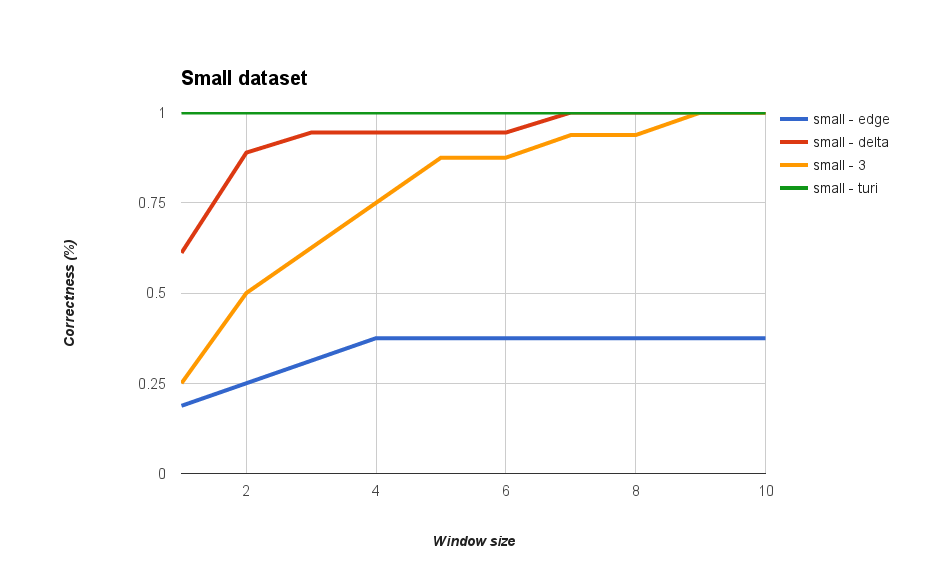
\includegraphics[width=\textwidth]{small.png}

\end{figure}
\end{frame}
% ------------------------------------------------------------------------------

% ------------------------------------------------------------------------------
\begin{frame}
\frametitle{Results: experiment 1}
\begin{figure}

	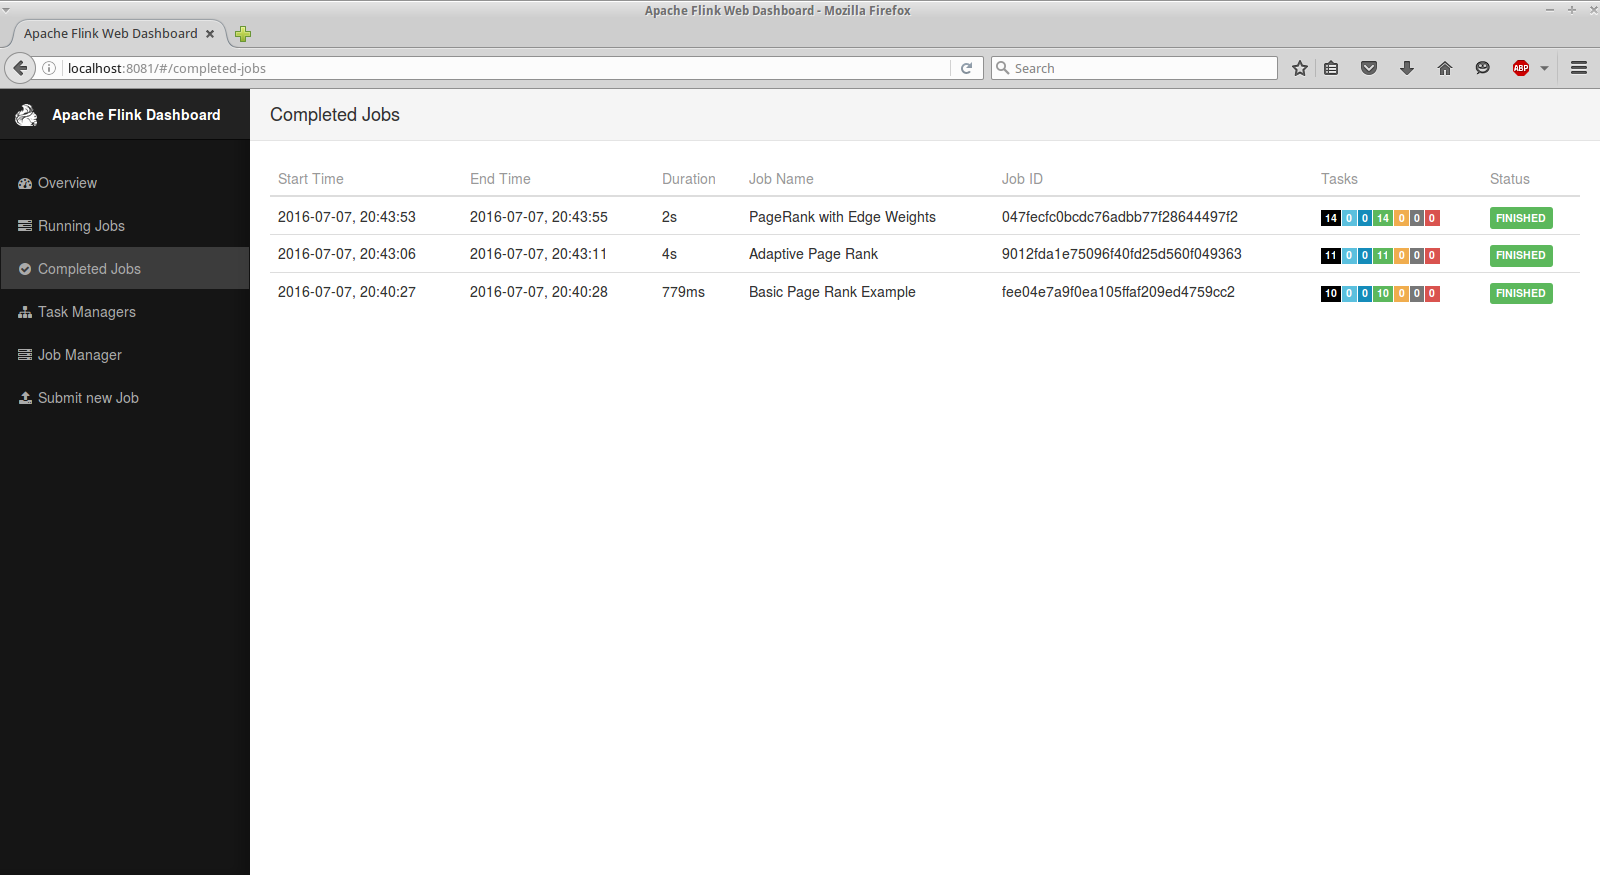
\includegraphics[width=\textwidth]{medium.png}

\end{figure}
\end{frame}
% ------------------------------------------------------------------------------

% ------------------------------------------------------------------------------
\begin{frame}
\frametitle{Results: experiment 1}
\begin{figure}

	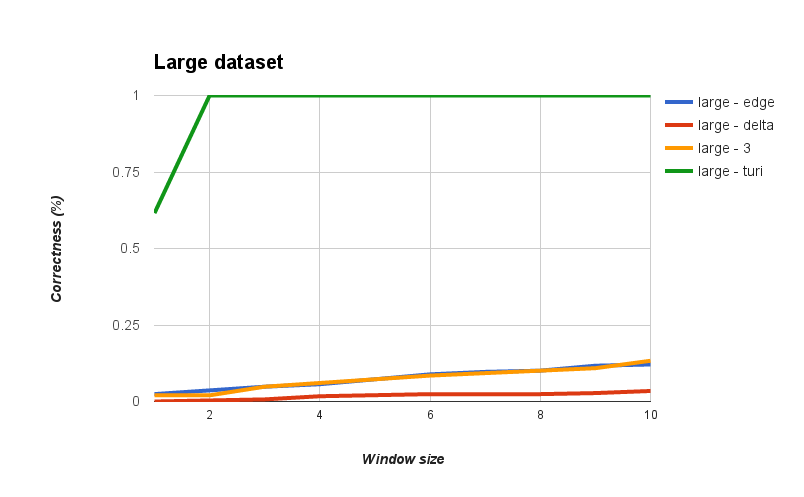
\includegraphics[width=\textwidth]{large.png}

\end{figure}
\end{frame}
% ------------------------------------------------------------------------------

% ------------------------------------------------------------------------------
\begin{frame}
\frametitle{Why are the results so bad?}
\begin{figure}

	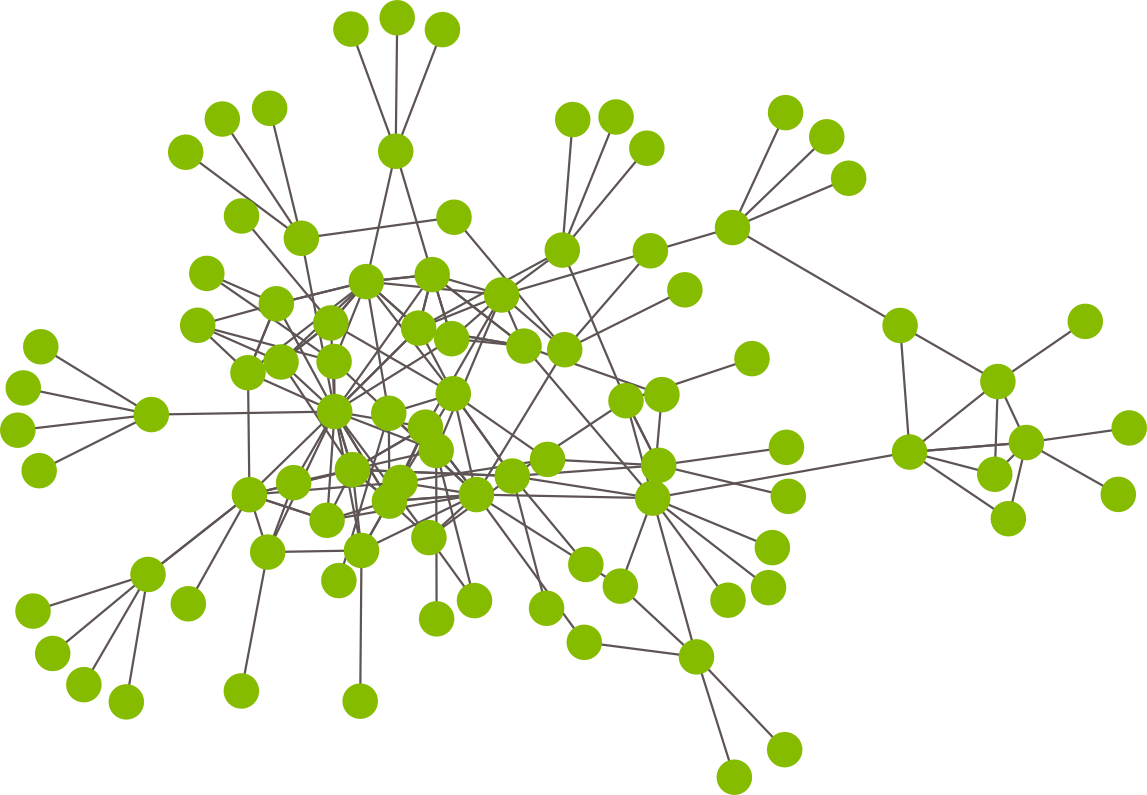
\includegraphics[width=\textwidth]{smallgraph.png}

\end{figure}
\end{frame}
% ------------------------------------------------------------------------------

% ------------------------------------------------------------------------------
\begin{frame}
\frametitle{Why are the results so bad?}
\begin{figure}

	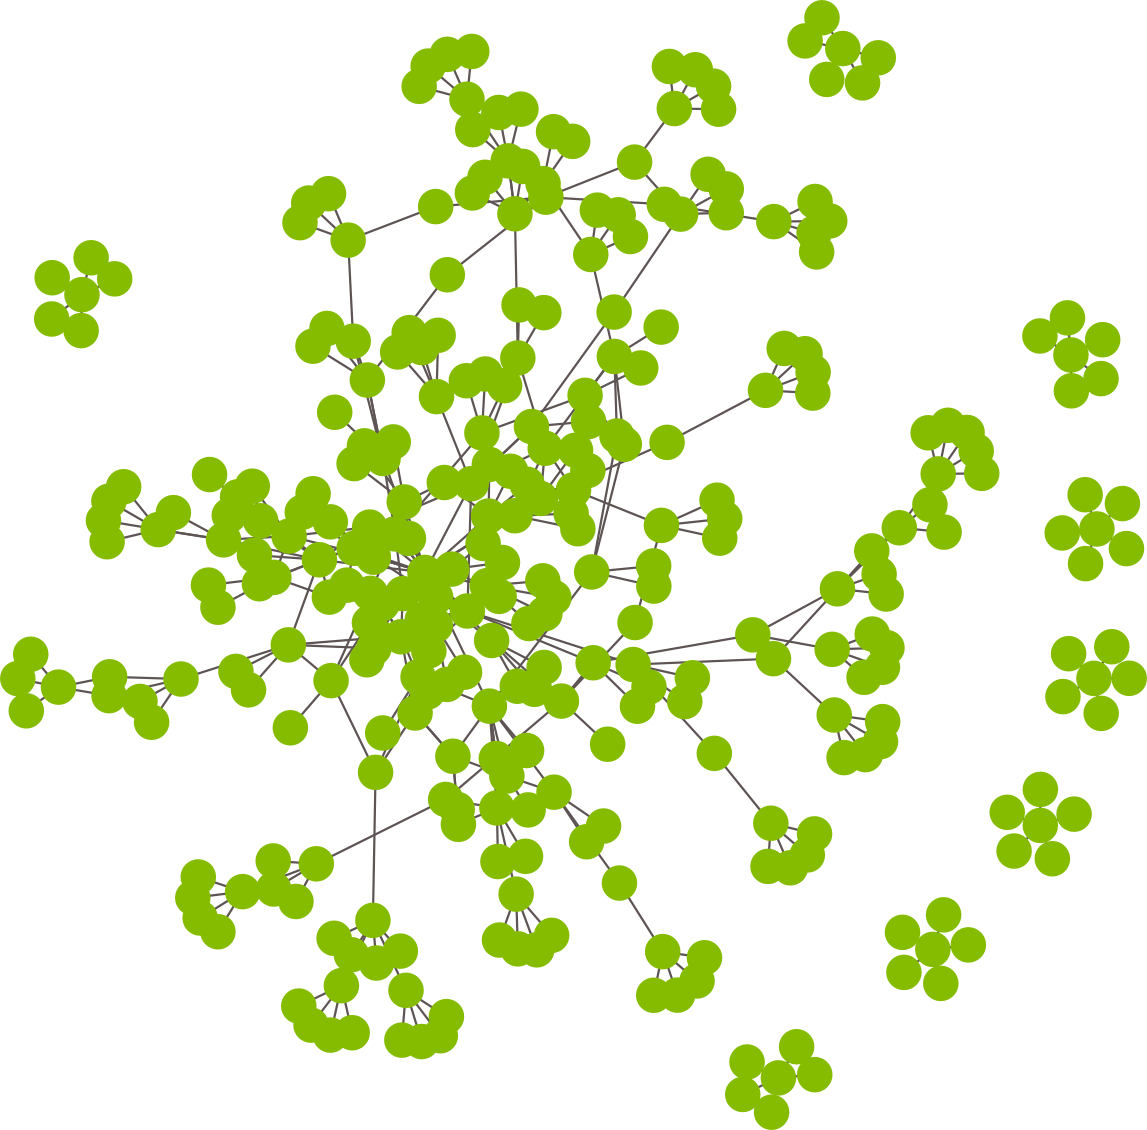
\includegraphics[width=0.7\textwidth]{mediumgraph.png}

\end{figure}
\end{frame}
% ------------------------------------------------------------------------------

% ------------------------------------------------------------------------------
\begin{frame}
\frametitle{Why are the results so bad?}
\begin{figure}

	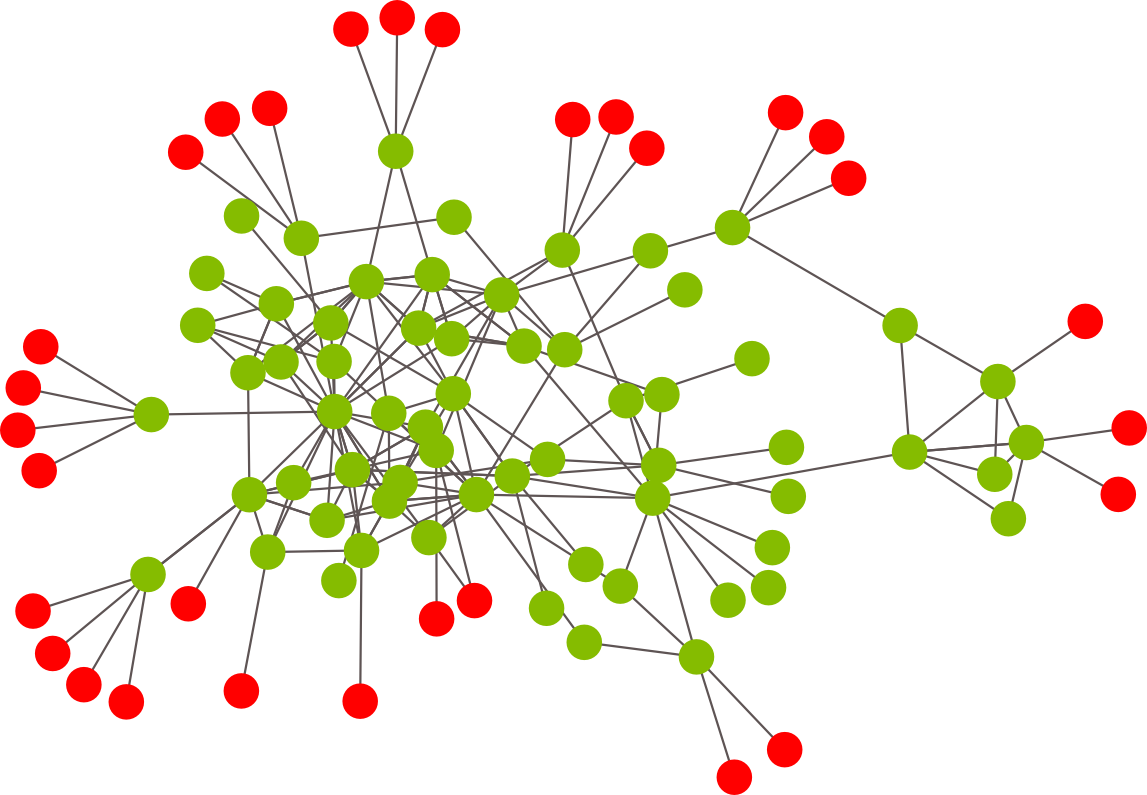
\includegraphics[width=\textwidth]{smallredgraph.png}

\end{figure}
\end{frame}
% ------------------------------------------------------------------------------

% ------------------------------------------------------------------------------
\begin{frame}
\frametitle{Why are the results so bad?}
\begin{figure}

	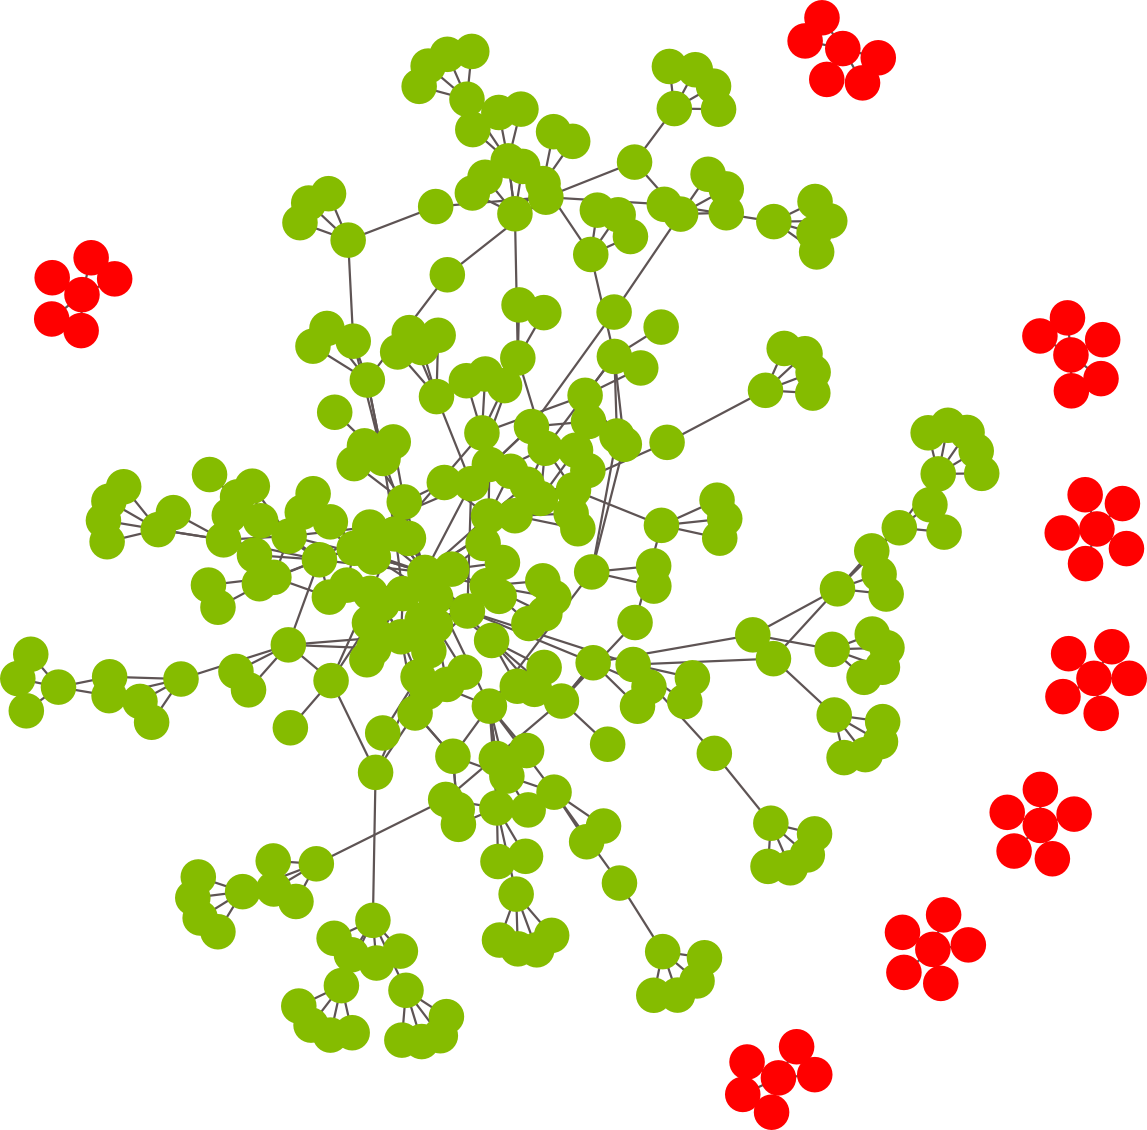
\includegraphics[width=0.7\textwidth]{mediumredgraph.png}

\end{figure}
\end{frame}
% ------------------------------------------------------------------------------
% ------------------------------------------------------------------------------
\begin{frame}
\frametitle{Speed of experiment 1}
\begin{figure}

	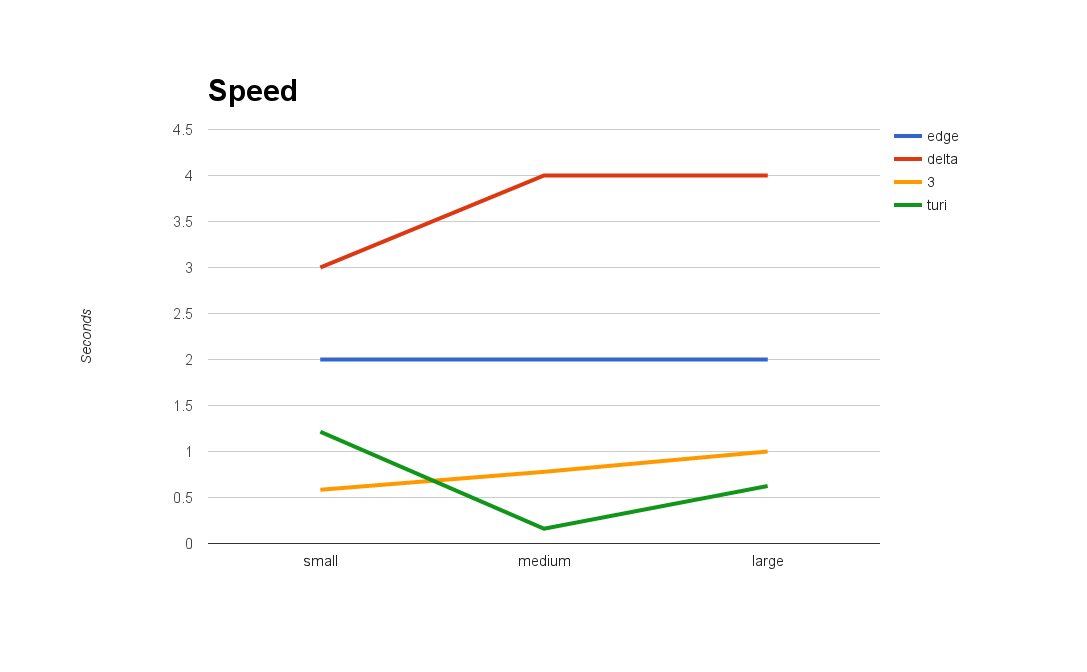
\includegraphics[width=\textwidth]{speeds.png}

\end{figure}
\end{frame}
% ------------------------------------------------------------------------------


% ------------------------------------------------------------------------------
\begin{frame}
\frametitle{Speed of experiment 2}
\begin{figure}

	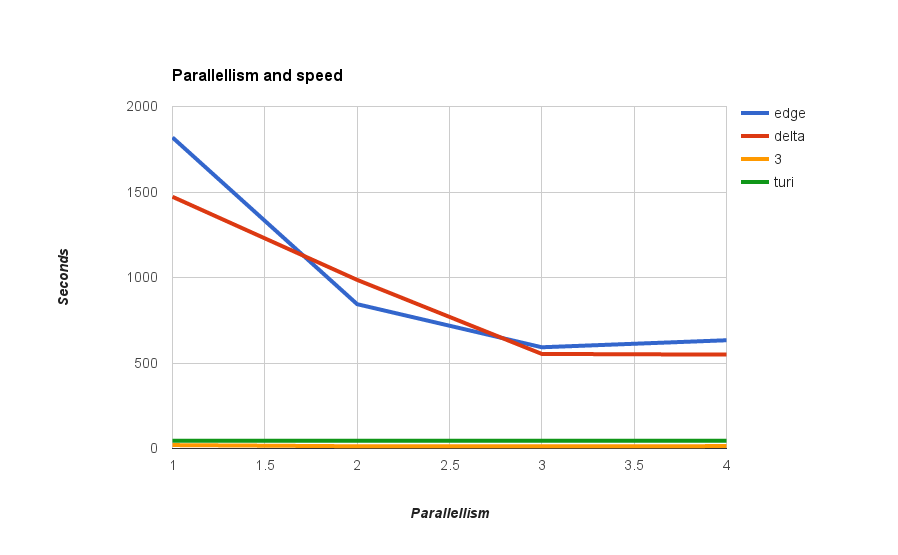
\includegraphics[width=\textwidth]{parallellism.png}

\end{figure}
\end{frame}
% ------------------------------------------------------------------------------

